\chapter{活的土壤}\label{ch:b2:living-soil}

达尔文去世前一年出版的最后一本书，
讲的是蚯蚓。1842 年，他在住所附近的一块田地上做了一个白垩标记，
1871 年将其挖出：标记埋在地下 18 厘米处，
被蚯蚓带到地表的蚓粪掩埋，
这一速率经他测量、称重并换算：每英亩每年有十吨
\omterm{def:b2:living-soil:soil}{土壤}经过蚯蚓的身体，以至于
“任何此类面积上的全部表层\omterm{def:b2:living-soil:soil}{土壤}，
都已经、并将每隔数年再次经过
蚯蚓的身体。”换言之，\omterm{def:b2:living-soil:soil}{土壤}并非生物立足其上的底物，
而是生物所造就的东西。本章讨论的正是这一造土过程：
岩石如何变成\omterm{def:b2:living-soil:soil}{土壤}、其过程多么缓慢，谁生活在其中、
数量几何，死去的物质如何被分解，
分解后留下什么，植物的根如何与真菌、
细菌进行交换，换取各自无法单独获得的养分，以及一块
历经万年才形成的\omterm{def:b2:living-soil:soil}{土壤}竟会以多快的速度流失。

\section{土壤是什么}

\begin{definition}[土壤及其土层]\label{def:b2:living-soil:soil}
\index{土壤}\index{土层}\index{腐殖质}\index{风化作用}\index{成土作用}
\emph{土壤}是覆盖陆地、支持植物生长的一层，由风化的矿物质、
有机物、水、空气和生物体组成。其体积约一半为孔隙，
孔隙中充满水或空气，比例随时变化，
固体部分为矿物颗粒——
砂（\qtyrange{0.05}{2}{mm}）、粉砂（\qtyrange{2}{50}{\micro m}）和
\omterm{prop:b2:living-soil:cec}{黏土}（小于 \qty{2}{\micro m}），其比例决定
\emph{质地}——另含百分之几的有机物，
它主导着土壤的大部分性质。土壤剖面中可见
\emph{土层}：表层的 \emph{O} 层为凋落物和部分分解的
有机物，位于表面；深色的 \emph{A} 层为矿质土，其中混有
\emph{腐殖质}，即分解产生的稳定、深色胶体残余物；
其下为 \emph{B} 层，\omterm{prop:b2:living-soil:cec}{黏土}、
铁和溶解的物质被淋入其中并在此积累；
\emph{C} 层为风化母岩，最底层为基岩。土壤
经\emph{成土作用}形成，取决于五个因素：母质、
气候、生物、地形和时间。土壤的形成极为缓慢，
风化每年产生约 \qty{0.1}{mm} 的
土壤，因此一米土壤相当于一万年的工作。
\end{definition}

\begin{omfigure}
\begin{tikzpicture}[every node/.style={font=\scriptsize}]
  \fill[brown!25!black!60] (0,5.4) rectangle (4,5.8); \node[right] at (4.2,5.6) {O：凋落物、苔藓、部分分解的有机物（几厘米）};
  \fill[brown!60!black] (0,4.2) rectangle (4,5.4); \node[right, align=left] at (4.2,4.8) {A：与腐殖质混合的矿质土，深色，团粒结构；\\ 大多数根系、大多数生物（\qtyrange{10}{30}{cm}）};
  \fill[brown!70!orange!80] (0,2.4) rectangle (4,4.2); \node[right, align=left] at (4.2,3.3) {B：黏土、氧化铁和碳酸盐的积累层，由上方淋洗而来 \\ 根系少（\qtyrange{30}{100}{cm}）};
  \fill[gray!50!brown!60] (0,1.0) rectangle (4,2.4); \node[right, align=left] at (4.2,1.7) {C：风化母岩，片段嵌于细粒基质中};
  \fill[gray!70] (0,0) rectangle (4,1.0); \node[right] at (4.2,0.5) {R：基岩};
  \foreach \x in {0.4,1.3,2.5,3.4} \draw[brown!30!black, thick] (\x,5.4) .. controls (\x+0.2,4.8) and (\x-0.2,4.4) .. (\x+0.1,3.6);
  \foreach \x/\y in {0.7/3.0, 2.0/2.7, 3.2/3.3, 1.5/1.6, 3.0/1.9} \fill[gray!80] (\x,\y) ellipse (0.18 and 0.1);
  \draw[<->, thick] (-0.4,5.8) -- (-0.4,0) node[midway, left, rotate=90, anchor=south] {约一至两米};
\end{tikzpicture}

{\small \omterm{def:b2:living-soil:soil}{土壤}剖面。有机物从顶部进入，随深度下降而被消耗；
矿物质在底部释放，
由根系和动物向上搬运；溶解物质随水向下迁移，
并在 B 层被截留。}
\end{omfigure}

\begin{proposition}[黏土和腐殖质为何重要]\label{prop:b2:living-soil:cec}
\index{阳离子交换容量}\index{黏土}\index{土壤结构}\index{田间持水量}
\omterm{prop:b2:living-soil:cec}{黏土}颗粒和\omterm{def:b2:living-soil:soil}{腐殖质}表面带负电荷，
并借静电吸引保有一定量可交换的
阳离子——$\mathrm{Ca^{2+}}$、$\mathrm{Mg^{2+}}$、$\mathrm{K^{+}}$、$\mathrm{NH_4^{+}}$——
植物根系通过释放 $\mathrm{H^{+}}$ 与之交换而取用它们。这一
\emph{\omterm{prop:b2:living-soil:cec}{阳离子交换容量}}是\omterm{def:b2:living-soil:soil}{土壤}的养分库；砂土
几乎没有（每千克仅几\omterm{def:b2:meiosis-heredity:linkage}{厘摩}尔电荷），黏壤土
富含\omterm{def:b2:living-soil:soil}{腐殖质}的黏壤土则多出五十倍，两者的肥力
因而相应不同。这些表面也能保持水分：砂质土
一天之内即排水至\emph{\omterm{prop:b2:living-soil:cec}{田间持水量}}（占其体积的十分之一），
壤土保持约三分之一，二者之差即作物
在两次降雨之间可利用的水分。\omterm{def:b2:living-soil:soil}{腐殖质}与真菌菌丝、
根系分泌物和蚯蚓黏液将矿物颗粒黏合成
\emph{团聚体}，即团粒结构，其孔隙使空气、水
和根系得以通过——这一性质使\omterm{def:b2:living-soil:soil}{土壤}有别于沉积物，
且它最先因耕翻和压实而遭破坏。
\end{proposition}

\section{谁生活在其中}

\begin{proposition}[土壤群落]\label{prop:b2:living-soil:community}
\index{土壤食物网}\index{食碎屑者}\index{蚯蚓}\index{土壤生物量}
每克肥沃表土中约有 $10^{9}$ 个细菌细胞，
分属约一万个物种，真菌菌丝长一百米，\omterm{def:b2:unicellular-diversity:protist}{原生生物} $10^{4}$ 个，
几十条线虫和一小撮螨类与
弹尾虫；每平方米有几百条蚯蚓，并且
在可见动物之下，活体生物量达每公顷数吨
——相当于同一公顷土地所能承载的牛群。
该群落是一个\emph{碎屑食物网}：细菌和真菌
（即\emph{分解者}）取食死亡物质，并被\omterm{def:b2:unicellular-diversity:protist}{原生生物}
和线虫（即微生物捕食者）被螨类和
捕食性线虫取食，后者又为蜈蚣和甲虫提供食物；
\emph{\omterm{prop:b2:living-soil:community}{食碎屑者}}——蚯蚓、马陆、鼠妇、白蚁、
弹尾虫等取食凋落物本身及其上的微生物，
将其切碎为千倍之多的碎片，并增加微生物
所攻击的表面。微生物捕食者的作用远超其数量：通过取食
细菌，释放出锁定在细菌细胞中的氮，形式为
铵；有\omterm{def:b2:unicellular-diversity:protist}{原生生物}和线虫的\omterm{def:b2:living-soil:soil}{土壤}，矿化
氮的速度快于仅有细菌的\omterm{def:b2:living-soil:soil}{土壤}。蚯蚓是
\emph{生态系统工程师}：它们的洞穴即\omterm{def:b2:living-soil:soil}{土壤}的
大孔，其蚓粪是最富集的团聚体，而
一片草地上的蚯蚓每年每公顷经其消化道
搬运约几吨\omterm{def:b2:living-soil:soil}{土壤}，正如达尔文所测定的。
\end{proposition}

\begin{omfigure}
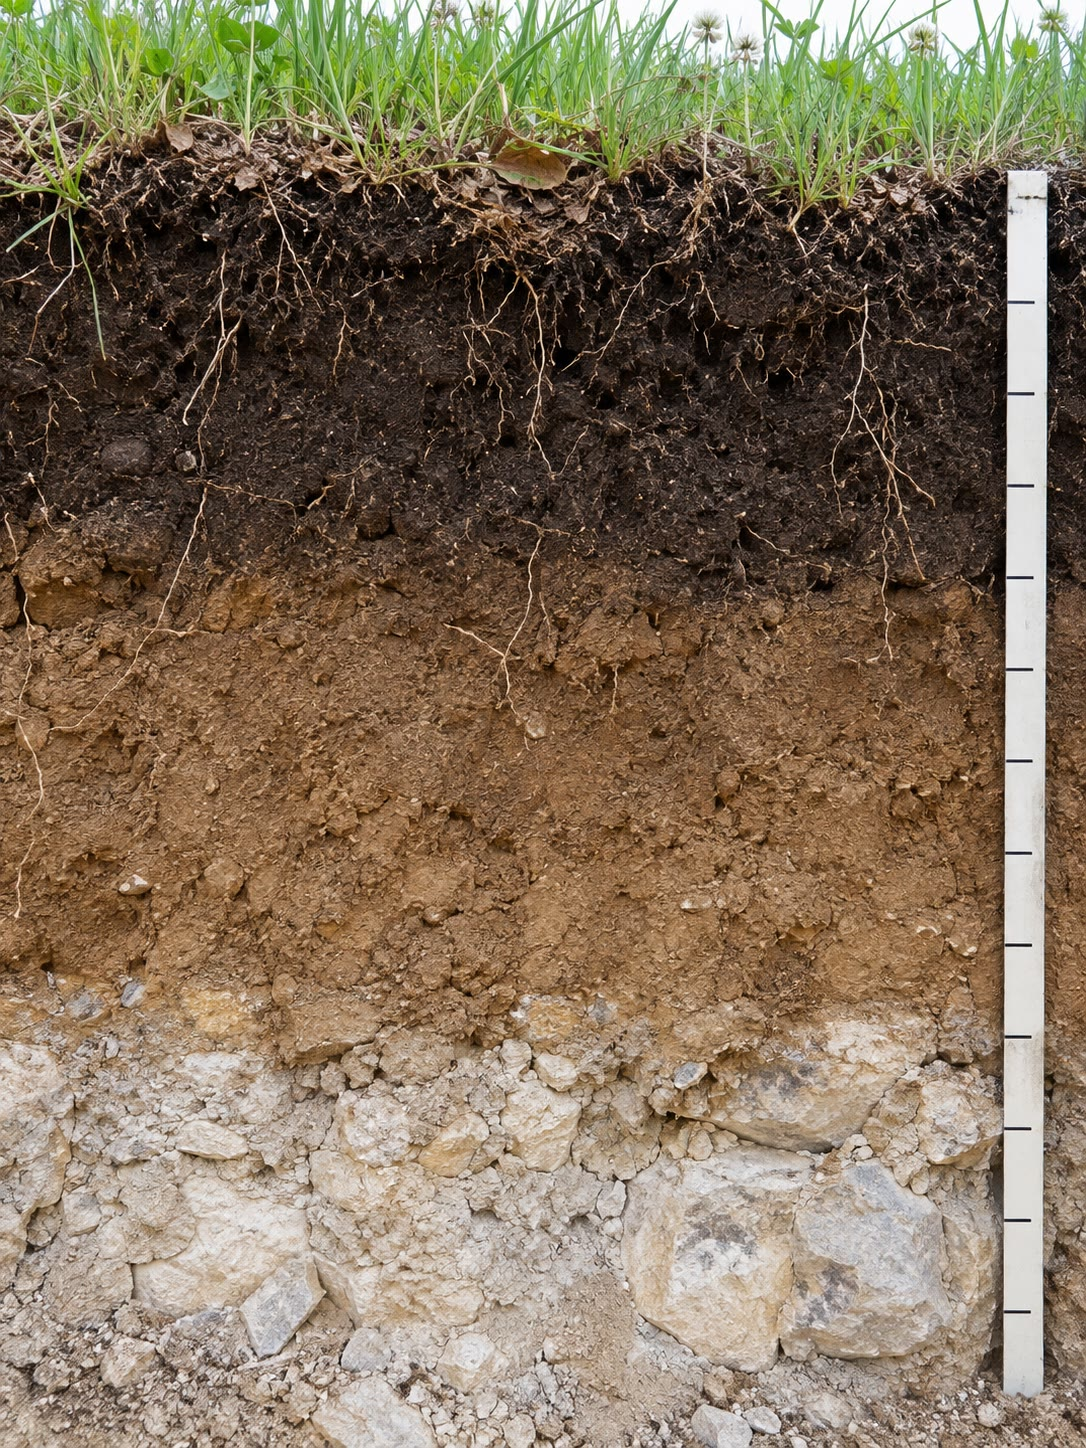
\includegraphics[width=0.21\linewidth]{images/book4/ai/b4-26-soil-profile.jpg}\hspace{0.025\linewidth}
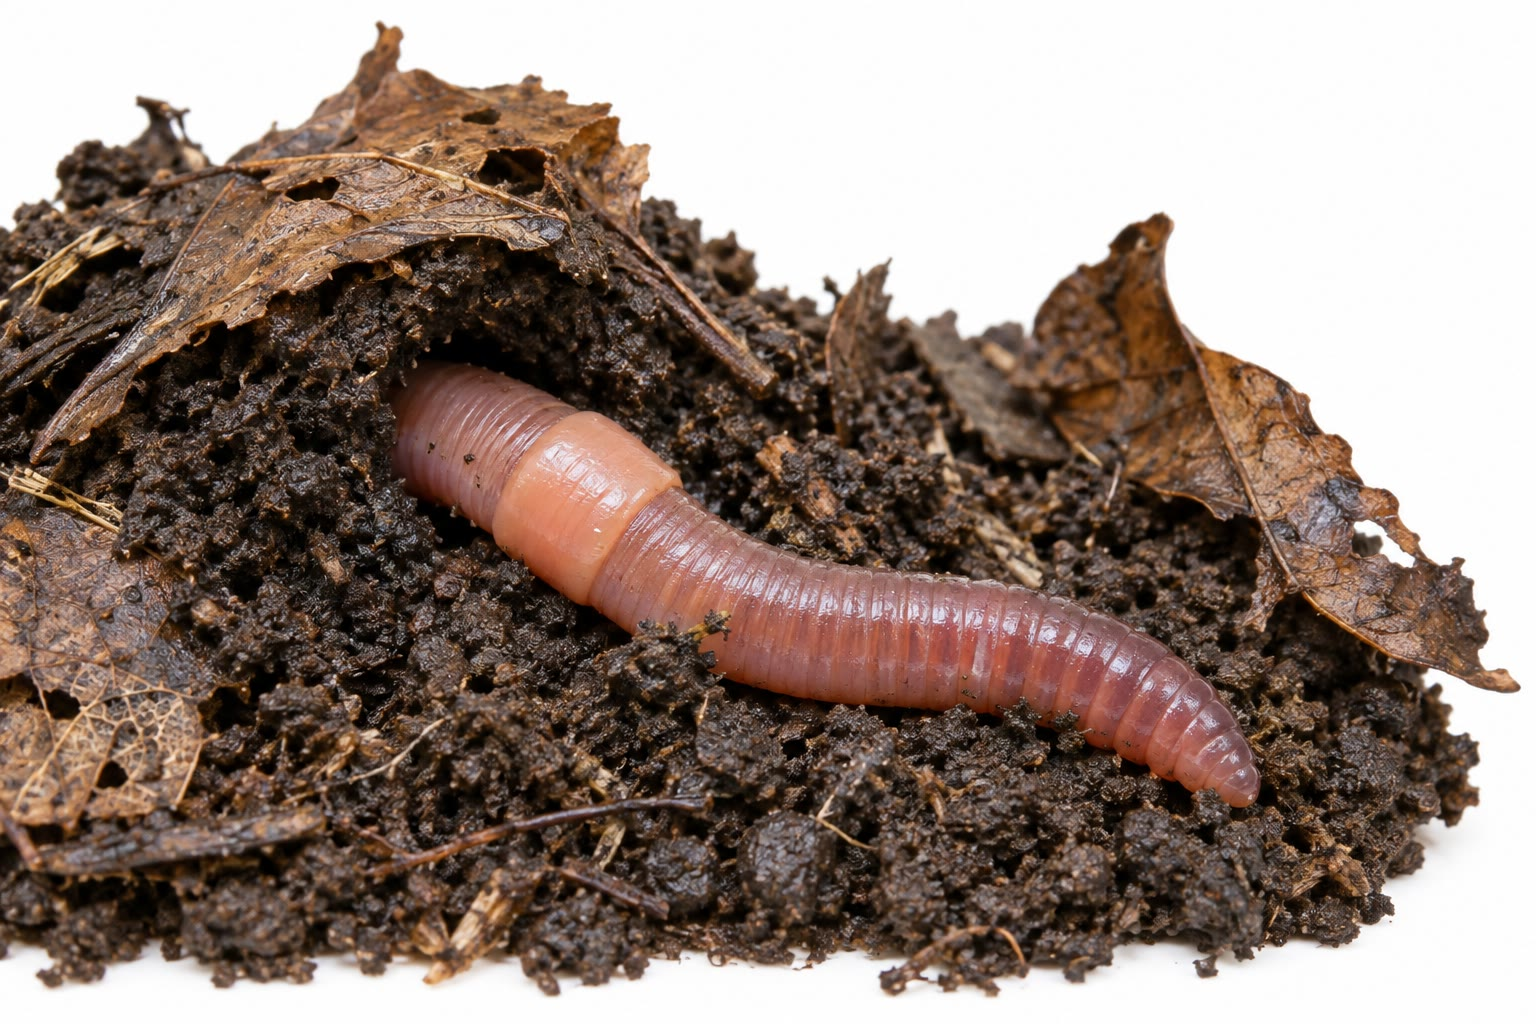
\includegraphics[width=0.42\linewidth]{images/book4/ai/b4-26-earthworm.jpg}\hspace{0.025\linewidth}
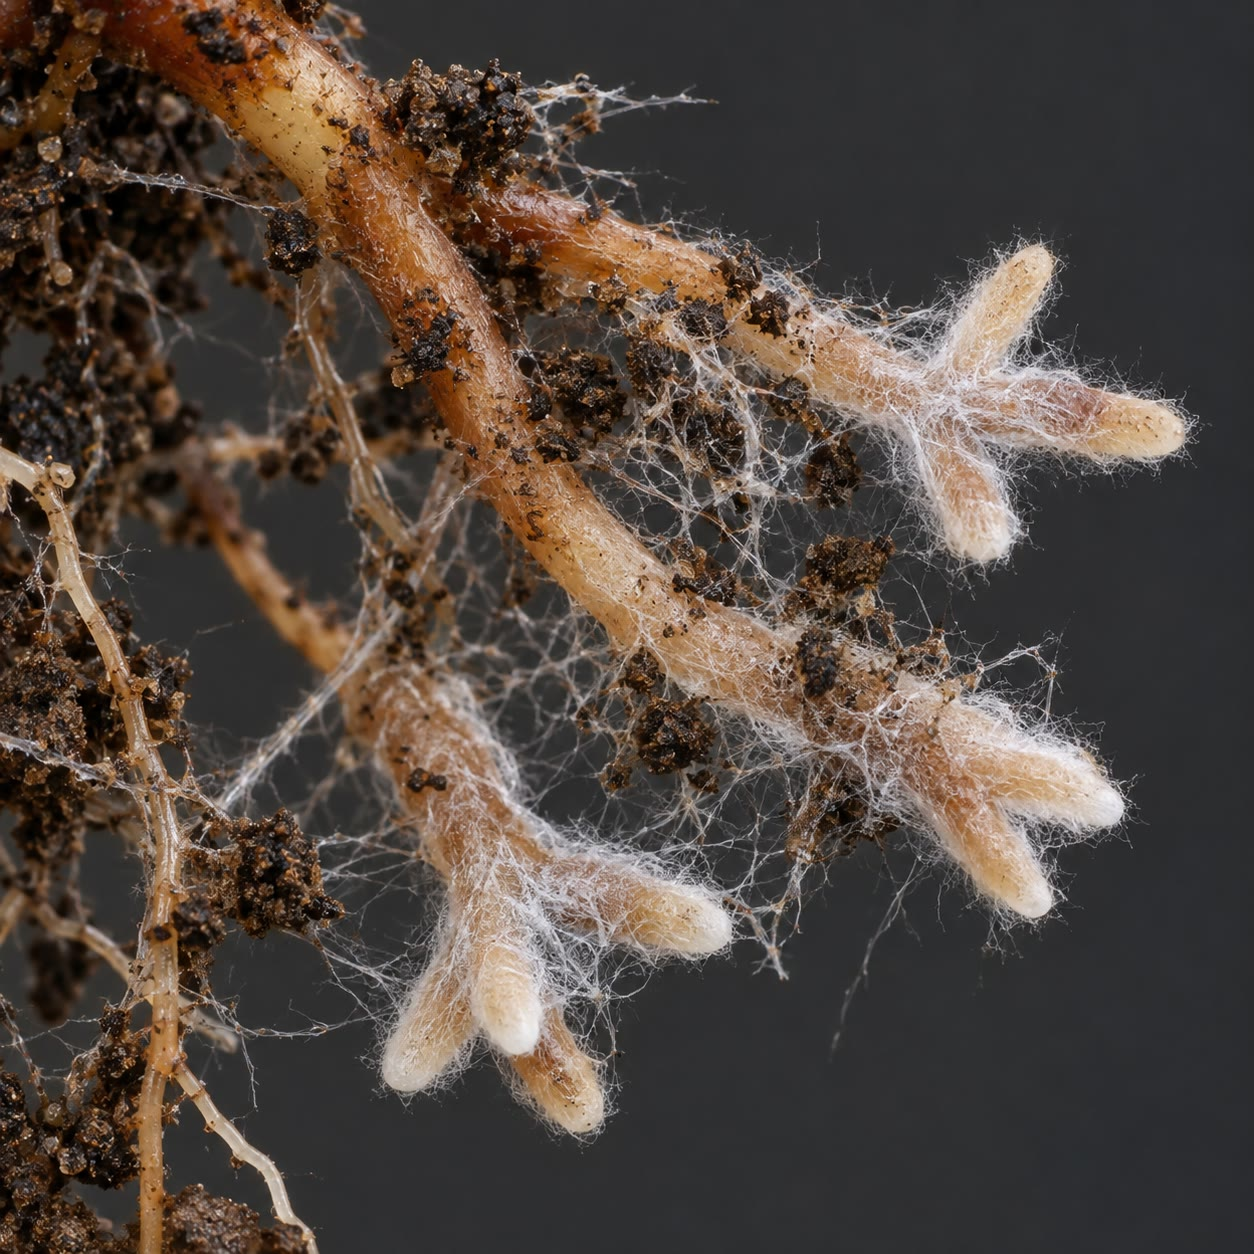
\includegraphics[width=0.28\linewidth]{images/book4/ai/b4-26-mycorrhiza.jpg}

{\small \omterm{def:b2:living-soil:soil}{土壤}及其两位“制造者”。左：切开的岸坡中的一个剖面，
深色表土向下渐变为浅色的风化岩。中间是
洞穴中的蚯蚓。右：一条根，及其外生菌根
鞘和伸入\omterm{def:b2:living-soil:soil}{土壤}的菌丝。}
\end{omfigure}

\section{分解}

\begin{theorem}[凋落物分解与碳氮比]\label{thm:b2:living-soil:decay}
\index{分解}\index{凋落物分解}\index{碳氮比}\index{矿化作用}\index{生物固持}
凋落物的分解速率与其剩余量成正比，
$\mathrm{d}L/\mathrm{d}t = -kL$，故 $L = L_0 e^{-kt}$，其中
\emph{衰变常数} $k$ 约为：草及温带森林落叶每年 1，
针叶 $0.3$，
湿润热带每年数个，苔原为 $0.05$；
稳定的年输入量 $I$ 会积累成量为 $I/k$ 的凋落物层。分解
受温度、湿度以及凋落物的
\emph{品质}：氮含量、木质素含量及
\omterm{thm:b2:living-soil:decay}{碳氮比}。微生物的 $\mathrm{C:N} \approx 8$，并
保留所摄入碳的约 \qty{40}{\%}，因此每
摄入 $8/0.4 = 20$ 个碳需要一个氮：凋落物 $\mathrm{C:N}$
低于约 25 时，分解过程中释放铵；
（\emph{\omterm{thm:b2:living-soil:decay}{矿化作用}}），而高于此值的凋落物——秸秆为 80，
\omterm{def:b2:plant-meristems:wood}{木材}为 400——则使微生物从\omterm{def:b2:living-soil:soil}{土壤}中吸收氮，
（\emph{\omterm{thm:b2:living-soil:decay}{生物固持}}），使植物缺氮，直至碳被呼吸掉、
比值降低为止。这正是新鲜秸秆翻耕入土会抑制作物的原因，
而豆科植物残体能为作物提供养分，
这也是堆肥需兼顾两者的原因。
\end{theorem}
\begin{proof}
比值的证明：食用每个氮含 $c$ 个碳的凋落物的
微生物同化 $0.4c$ 个碳，为以 $\mathrm{C:N} = 8$ 构建生物量，
需要 $0.4c/8 = c/20$ 个氮；凋落物
仅提供 1 个。若 $c < 20$，则氮有剩余，以
铵的形式释放；若 $c > 20$，则缺口由\omterm{def:b2:living-soil:soil}{土壤}补足。
实际中阈值 25 反映的保留效率略低于
0.4。对凋落物层，$\mathrm{d}L/\mathrm{d}t = I - kL$
\omterm{def:b2:biogeochemical-cycles:reservoir}{稳态}为 $I/k$，以时间常数 $1/k$ 趋近\omterm{def:b2:biogeochemical-cycles:reservoir}{稳态}；凋落物的
\omterm{def:b2:biogeochemical-cycles:reservoir}{停留时间}为 $1/k$，山毛榉林中为一年，
苔原中为二十年。
\end{proof}
\begin{proof}[证据]
凋落物袋实验——将已知质量的叶片装入网袋，
埋入土中并定期称重——得出了指数规律及其
在各生物群系中的常数（奥尔森，1963），并以不同网孔大小表明，
排除\omterm{def:b2:living-soil:soil}{土壤}动物会使分解速率减半：微生物
负责化学过程，动物则决定节奏。
在一大洲范围内，同一种叶片在佐治亚州一年即分解，
在阿拉斯加需八年，分解速率与实际蒸散量成正比，
即温度与水分的乘积。
\end{proof}

\begin{omfigure}
\begin{tikzpicture}
\begin{axis}[
  width=0.72\linewidth, height=5.6cm,
  axis x line=bottom, axis y line=left,
  xmin=0, xmax=6, ymin=0, ymax=105,
  xlabel={年}, ylabel={剩余凋落物质量 (\%)},
  xlabel style={font=\small, at={(axis description cs:0.5,-0.13)}, anchor=north},
  ylabel style={font=\small},
  tick label style={font=\small},
  legend style={font=\scriptsize, at={(0.5,-0.3)}, anchor=north, draw=none, legend columns=2},
  clip=false,
]
\addplot[very thick, omDef, domain=0:6, samples=60] {100*exp(-2*x)};
\addlegendentry{热带雨林叶片，$k = 2$}
\addplot[very thick, omThm, domain=0:6, samples=60] {100*exp(-1*x)};
\addlegendentry{山毛榉叶，$k = 1$}
\addplot[very thick, omProp, domain=0:6, samples=60] {100*exp(-0.3*x)};
\addlegendentry{云杉针叶，$k = 0.3$}
\addplot[very thick, gray, domain=0:6, samples=60] {100*exp(-0.05*x)};
\addlegendentry{苔原苔藓，$k = 0.05$}
\end{axis}
\end{tikzpicture}

{\small 凋落物的指数衰减。山毛榉叶减半需
八个月；苔原\omterm{def:b2:plant-life-cycles:moss}{苔藓}减半需十四年；
微生物和动物都无法分解完的残余，即成为\omterm{def:b2:living-soil:soil}{腐殖质}。}
\end{omfigure}

\begin{proposition}[腐殖质与土壤碳库]\label{prop:b2:living-soil:humus}
\index{腐殖质}\index{土壤有机碳}\index{土壤呼吸}
凋落物碳中有百分之几逃脱了彻底氧化，
并转化为\emph{\omterm{def:b2:living-soil:soil}{腐殖质}}：一种深色、无定形的混合物，由微生物残体、
改性木质素及植物化合物组成，与\omterm{prop:b2:living-soil:cec}{黏土}和铁结合，
并被包裹于团聚体之中，其分解的\omterm{def:b2:biogeochemical-cycles:reservoir}{停留时间}为
数十年至数千年。\omterm{def:b2:living-soil:soil}{腐殖质}是\omterm{def:b2:living-soil:soil}{土壤}肥力的所在，
——大部分氮和\omterm{prop:b2:living-soil:cec}{阳离子交换容量}、一半的持水能力都在其中，
并且它是陆地上最大的有机碳库，
在表层一米内为 \qty{1700}{GtC}，是大气的两倍。其
平衡由输入减去分解决定，$\mathrm{d}H/\mathrm{d}t = I_h - k_hH$：
当 $k_h \approx 0.02$ 每年时，\omterm{def:b2:living-soil:soil}{土壤}保留相当于五十年输入的
任何变化——翻耕会破坏团聚体，
并使\omterm{def:b2:living-soil:soil}{腐殖质}通气；泥炭排水会引入氧气；
增温会提高 $k_h$——这些变化都表现为一种持续
数十年的损失。全球耕地\omterm{def:b2:living-soil:soil}{土壤}自开垦以来已失去三分之一至一半的
\omterm{def:b2:living-soil:soil}{腐殖质}，其中约
\qty{100}{GtC}；升温 \qty{3}{\celsius} 将使其余部分的分解
速率提高三分之一：\omterm{def:b2:living-soil:soil}{土壤}是
在\cref{ch:b2:global-change}中碳收支最大的不确定因素。
\end{proposition}

\section{地下的伙伴关系}

\begin{proposition}[菌根与根瘤菌]\label{prop:b2:living-soil:symbiosis}
\index{菌根}\index{根瘤菌}\index{根瘤}\index{固氮酶}\index{豆血红蛋白}
十种植物中有九种的根被真菌定殖，形成
\emph{菌根}：植物提供糖（约占其
光合产物的十分之一至五分之一），真菌则提供磷酸盐、氮、水和
锌，其菌丝比根细一百倍，并
每单位碳延伸的长度为其自身的百倍，从
根所不能到达的\omterm{def:b2:living-soil:soil}{土壤}体积中收集养分——尤其是磷酸盐，
磷酸盐在\omterm{def:b2:living-soil:soil}{土壤}中扩散极慢，以至于根
在数天内即耗尽其周围一毫米的范围。
\emph{丛枝菌根}，较古老的一类，进入根细胞
并分枝形成丛枝，物质交换在此发生；
\emph{外生菌根}见于森林树木，包裹根尖，
并在其细胞之间生长。豆科植物则更进一步：\omterm{prop:b2:living-soil:symbiosis}{根瘤菌}受根的类黄酮吸引，
经\omterm{prop:b2:plant-meristems:ram}{根毛}侵入，根
围绕它们形成\emph{\omterm{prop:b2:living-soil:symbiosis}{根瘤}}，细菌在其中以
\emph{类菌体}形式，借助\omterm{prop:b2:living-soil:symbiosis}{固氮酶}固定氮——这是一种对氧极为敏感的酶，
以至于\omterm{prop:b2:living-soil:symbiosis}{根瘤}必须靠
\emph{\omterm{prop:b2:living-soil:symbiosis}{豆血红蛋白}}（植物所产生的一种血红蛋白）维持近乎无氧的环境，它
使\omterm{prop:b2:living-soil:symbiosis}{根瘤}呈粉红色，并向类菌体输送氧，
其浓度低到不会毒害该酶。双方
相互监督：植物会切断对不\omterm{prop:b2:biogeochemical-cycles:nitrogen}{固氮}\omterm{prop:b2:living-soil:symbiosis}{根瘤}的
供糖，输送磷酸盐较少的真菌也
只能获得较少的碳。
\end{proposition}
\begin{proof}[证据]
基尔斯及其同事（2011）让一株植物与两种真菌伙伴
在分根系统中培养，仅向一侧提供磷酸盐：
植物向供应磷酸盐更多的真菌分配更多的碳，
真菌则向给予更多碳的根分配更多磷酸盐
——这种互惠回报由同位素测定。
就\omterm{prop:b2:living-soil:symbiosis}{根瘤}而言，实验中被剥夺氮素的\omterm{prop:b2:living-soil:symbiosis}{根瘤}（
以氩气和氧气替代空气），获得的氧较少，
生长也比同一植株上能\omterm{prop:b2:biogeochemical-cycles:nitrogen}{固氮}的\omterm{prop:b2:living-soil:symbiosis}{根瘤}弱：植物
会惩罚“搭便车者”。氮-15 示踪表明，三叶草与禾草
草地在一个生长季内，将三叶草所固定氮的三分之一转移给
禾草，途经\omterm{def:b2:living-soil:soil}{土壤}和共享的真菌
网络。
\end{proof}

\begin{omfigure}
\begin{tikzpicture}[every node/.style={font=\scriptsize}, >=stealth]
  % root cross-section
  \fill[omThm!15] (0,0) circle (1.5); \draw[thick] (0,0) circle (1.5);
  \fill[omThm!30] (0,0) circle (0.5); \draw[thick] (0,0) circle (0.5);
  \node at (0,0) {中柱};
  \node at (0,1.05) {皮层};
  % arbuscules in cortex cells
  \foreach \a in {30,150,270} { \draw[omDef, thick] ({1.0*cos(\a)},{1.0*sin(\a)}) -- ++({0.25*cos(\a+60)},{0.25*sin(\a+60)}) -- ++({0.2*cos(\a-40)},{0.2*sin(\a-40)}); \draw[omDef, thick] ({1.0*cos(\a)},{1.0*sin(\a)}) -- ++({0.25*cos(\a-60)},{0.25*sin(\a-60)}); }
  % hyphae out
  \foreach \a in {20,80,150,210,340} { \draw[omDef, thick] ({1.5*cos(\a)},{1.5*sin(\a)}) .. controls ({2.2*cos(\a+10)},{2.2*sin(\a+10)}) .. ({2.7*cos(\a-5)},{2.7*sin(\a-5)}); }
  \draw[omDef, thick] ({1.5*cos(150)},{1.5*sin(150)}) -- ({1.0*cos(150)},{1.0*sin(150)});
  \node[omDef, anchor=west, align=left] at (2.9,1.4) {菌丝：宽 \qty{3}{\micro m}，\\ 每厘米根的菌丝长（米）};
  \node[omDef, anchor=west] at (2.9,0.1) {皮层细胞内的丛枝};
  \draw[omDef] (2.85,0.1) -- (1.2,0.5);
  \node[anchor=north, align=center] at (0,-1.6) {根，直径 \qty{0.3}{mm}};
  \draw[->, thick, omThm] (-1.2,-2.4) -- (1.2,-2.4) node[right] {糖分流向真菌，占光合产物的 \qtyrange{10}{20}{\%}};
  \draw[<-, thick, omDef] (-1.2,-2.9) -- (1.2,-2.9) node[right] {磷酸盐、铵、水和锌流向植物};
  % nodule
  \begin{scope}[xshift=9.3cm]
    \draw[thick, brown!60!black] (-0.3,2.4) -- (-0.1,-0.6);
    \draw[thick, brown!60!black] (-0.1,0.3) -- (1.6,0.1);
    \fill[pink!60!red!40] (1.5,0.2) circle (0.9); \draw[thick] (1.5,0.2) circle (0.9);
    \fill[pink!80!red!60] (1.5,0.2) circle (0.55);
    \foreach \p in {(1.3,0.3),(1.6,0.0),(1.5,0.45),(1.7,0.3),(1.35,0.05)} \fill[omDef!70!black] \p ellipse (0.08 and 0.05);
    \node[anchor=north, align=center] at (1.5,-0.8) {根瘤：植物细胞中的类菌体，\\ 因含豆血红蛋白而呈粉红色；\\ 氧气维持在 \qty{10}{nM}，既使固氮酶 \\ 能工作，细胞又能进行呼吸};
    \node[anchor=south, align=center] at (-0.2,2.45) {豆科植物根};
  \end{scope}
\end{tikzpicture}

{\small 两笔互利交易。左：丛枝菌根，糖分向外输出，
磷酸盐经皮层细胞内的丛枝向内输入。右：
豆科植物\omterm{prop:b2:living-soil:symbiosis}{根瘤}，其中植物自身的血红蛋白使
氧气水平既足以保护\omterm{prop:b2:living-soil:symbiosis}{固氮酶}，又足以供呼吸。}
\end{omfigure}

\section{土壤流失}

\begin{proposition}[侵蚀、盐渍化与土壤平衡]\label{prop:b2:living-soil:erosion}
\index{土壤侵蚀}\index{盐渍化}\index{荒漠化}
\omterm{def:b2:living-soil:soil}{土壤}每年以 \qtyrange{0.05}{0.5}{mm} 的速度形成，在自然植被下，
其侵蚀速率与之大致相当。裸露的耕地位于
坡面上，每年因水和风损失 \qtyrange{1}{10}{mm}——
\qtyrange{10}{100}{t/ha}——相当于形成速率的十至一百倍：
一万年形成的\omterm{def:b2:living-soil:soil}{土壤}，一个世纪内便被
冲走，连同 A 层的\omterm{def:b2:living-soil:soil}{腐殖质}和养分，
而这正是唯一要紧的部分。覆盖作物、梯田、等高耕作，
以及免耕法，即让残茬留在地表，使团聚体
保持完整，使流失量回到接近形成速率的水平。
干旱气候下的灌溉则带来相反的问题：水
蒸发后留下盐分，每公顷每年约一吨，盐分来自
仅微咸的水，直至\omterm{def:b2:living-soil:soil}{土壤}溶液
（见\cref{ch:b2:plant-plasticity}）的渗透势低于根系
所能克服的程度——\emph{\omterm{prop:b2:living-soil:erosion}{盐渍化}}，使苏美尔的
农田于四千年前即被废弃，如今影响着约五分之一的
灌溉土地。\omterm{def:b2:living-soil:soil}{土壤}的状况是一本收支账：\omterm{def:b2:living-soil:soil}{腐殖质}输入对
输出、形成对侵蚀、盐分输入对
排出；每一项都有\omterm{def:b2:biogeochemical-cycles:reservoir}{停留时间}，且一旦为负，
便难以逆转。
\end{proposition}

\section{练习}

\begin{exercise}[$\star$]\label{exo:b2:living-soil:1}
自地表向下列出\omterm{def:b2:living-soil:soil}{土壤}剖面的各\omterm{def:b2:living-soil:soil}{土层}，并说明
每一层中发生的变化。
\end{exercise}

\begin{exercise}[$\star$]\label{exo:b2:living-soil:2}
解释什么是\omterm{prop:b2:living-soil:cec}{阳离子交换容量}，并说明砂质\omterm{def:b2:living-soil:soil}{土壤}为何
该容量很小，以及农民给酸性\omterm{def:b2:living-soil:soil}{土壤}施石灰时对其做了什么。
\end{exercise}

\begin{exercise}[$\star$]\label{exo:b2:living-soil:3}
列出\omterm{prop:b2:living-soil:community}{土壤食物网}中的主要类群，自分解者至顶级
捕食者，每类各举一例，并说明摄食细菌的生物
对植物起什么作用。
\end{exercise}

\begin{exercise}[$\star$]\label{exo:b2:living-soil:4}
区分丛枝菌根与外生菌根，并说明二者各
自提供什么、获得什么。
\end{exercise}

\begin{exercise}[$\star\star$]\label{exo:b2:living-soil:5}
一片山毛榉林每年落下 \qty{4}{t/ha} 的树叶，其凋落物
凋落物以 $k = 0.8$ 每年的速率分解。求\omterm{def:b2:biogeochemical-cycles:reservoir}{稳态}凋落物
质量、凋落物的\omterm{def:b2:biogeochemical-cycles:reservoir}{停留时间}，以及一年落叶
损失 \qty{90}{\%} 质量所需的时间。
\end{exercise}

\begin{exercise}[$\star\star$]\label{exo:b2:living-soil:6}
小麦秸秆的 $\mathrm{C:N} = 80$，三叶草残茬为 $15$。对
各自计算微生物每消耗 \qty{100}{kg}
碳所需的氮（保留率 0.4，微生物 $\mathrm{C:N} = 8$），并
判断残茬是矿化还是被固持，并求其数量。
\end{exercise}

\begin{exercise}[$\star\star$]\label{exo:b2:living-soil:7}
一公顷草地含有 \qty{2}{t} 蚯蚓，它们每年
各自处理的\omterm{def:b2:living-soil:soil}{土壤}为自身质量的十倍。求每年经蚯蚓
处理的\omterm{def:b2:living-soil:soil}{土壤}量，以及表层
\qty{20}{cm}（容重 \qty{1.3}{t/m^3}）全部通过一次所需的时间。
与达尔文的数值相比较。
\end{exercise}

\begin{exercise}[$\star\star$]\label{exo:b2:living-soil:8}
每克\omterm{def:b2:living-soil:soil}{土壤}含有 $10^{9}$ 个细菌，每个细菌质量为 \qty{e-12}{g}，
另有 \qty{100}{m} 菌丝，直径为 \qty{4}{\micro m}，密度为
\qty{1.1}{g/cm^3}。求每克\omterm{def:b2:living-soil:soil}{土壤}中细菌与真菌的生物量，
以及每公顷的生物量（表层 \qty{20}{cm}，\qty{1.3}{t/m^3}）。
\end{exercise}

\begin{exercise}[$\star\star$]\label{exo:b2:living-soil:9}
\omterm{def:b2:living-soil:soil}{土壤}\omterm{def:b2:living-soil:soil}{腐殖质}以每年 $k_h = 0.02$ 的速率分解，每年
输入 \qty{1.5}{t/ha} 的碳。求\omterm{def:b2:biogeochemical-cycles:reservoir}{稳态}时\omterm{def:b2:living-soil:soil}{腐殖质}的
碳量。田地翻耕后 $k_h$ 加倍，求新的\omterm{def:b2:biogeochemical-cycles:reservoir}{稳态}、
损失的碳量，以及损失一半所需的时间。
\end{exercise}

\begin{exercise}[$\star\star\star$]\label{exo:b2:living-soil:10}
磷酸盐在\omterm{def:b2:living-soil:soil}{土壤}中以 $D \approx \qty{e-13}{m^2/s}$ 扩散。
求其在 \num{100} 天的生长季内扩散的距离，
（$x \approx \sqrt{2Dt}$），并与根的间距
（\qty{1}{cm}）和菌丝的间距（\qty{0.1}{mm}）相比较。这说明
为什么菌根对磷的意义大于对硝酸盐的意义
（$D \approx \qty{e-10}{m^2/s}$）？
\end{exercise}

\begin{exercise}[$\star\star\star$]\label{exo:b2:living-soil:11}
某坡地每年因侵蚀损失 \qty{20}{t/ha} \omterm{def:b2:living-soil:soil}{土壤}，
同时形成 \qty{1}{t/ha}。A 层厚 \qty{25}{cm}，
容重 \qty{1.3}{t/m^3}，含碳 \qty{3}{\%}。求 A 层的质量、
按此速率计算的寿命，以及每年损失的碳量。若
改为免耕，损失降至 \qty{2}{t/ha}，
则重新计算其寿命。
\end{exercise}

\begin{exercise}[$\star\star\star$]\label{exo:b2:living-soil:12}
“\omterm{def:b2:living-soil:soil}{土壤}是农场里最慢的生物。”结合
凋落物、\omterm{def:b2:living-soil:soil}{腐殖质}、矿质\omterm{def:b2:living-soil:soil}{土壤}和盐分的\omterm{def:b2:biogeochemical-cycles:reservoir}{停留时间}进行讨论，
并说明农民在一生中能看到哪些变化，哪些则看不到。
\end{exercise}

\section{问题：一公顷土壤}

\begin{problem}[{周末问题——一公顷耕地土壤的核算：统计其
活体质量，依据指数收支追踪凋落物和腐殖质，
计算豆科植物残体释放的氮与作物需求，
比较两种管理方式下的侵蚀与碳账目，
最后给出土壤的碳储量、翻耕下的
寿命，以及豆科植物
提供的氮}]
\label{pb:b2:living-soil:1}
本公顷土地：A 层厚 \qty{25}{cm}，容重 \qty{1.3}{t/m^3}，
有机碳含量 \qty{2.5}{\%}；翻耕条件下\omterm{def:b2:living-soil:soil}{腐殖质}分解速率 $k_h =
0.025$ 每年，免耕条件下为 $0.015$；两种情况下每年输入
\omterm{def:b2:living-soil:soil}{腐殖质}的碳均为 \qty{1.2}{t/ha}。凋落物：一种三叶草覆盖作物
留下 \qty{5}{t/ha} 干物质，碳含量 \qty{45}{\%}，氮含量
\qty{3}{\%}，分解速率 $k = 2$ 每年。侵蚀：翻耕时每年
\qty{15}{t/ha}，免耕时 \qty{1.5}{t/ha}；成土速率
\qty{0.5}{t/ha}。

\medskip
\noindent\textbf{第一部分——储量。}
\begin{enumerate}
  \item 计算 A 层的质量及其有机碳量。
  \item 计算\omterm{def:b2:living-soil:soil}{腐殖质}中的氮质量，若其
        $\mathrm{C:N}$ 为 12。
  \item \omterm{def:b2:living-soil:soil}{土壤}每克含 $10^{9}$ 个细菌，每个质量为 \qty{e-12}{g}，
        每克含 \qty{200}{m} 菌丝，
        直径为 \qty{4}{\micro m}，密度为 1.1，
        计算每公顷的微生物生物量。
  \item 加上 \qty{1.5}{t/ha} 的蚯蚓和 \qty{0.2}{t/ha} 的
        其他动物，给出每公顷的活体总质量，
        它占\omterm{def:b2:living-soil:soil}{腐殖质}碳量的比例是多少？
  \item 微生物每年周转其生物量两次，
        并呼吸消耗其所摄取物质的 \qty{60}{\%}，
        估算其每年消耗的碳量，以及释放的 $\mathrm{CO_2}$。
  \item 与作物的净初级生产量相比较，其量约为
        \qty{5}{t/ha} 碳，并加以评论。
\end{enumerate}

\medskip
\noindent\textbf{第二部分——三叶草残体。}
\begin{enumerate}[resume]
  \item 计算残体中的碳和氮，以及其
        $\mathrm{C:N}$。
  \item 若微生物的 $\mathrm{C:N} = 8$，留存率为 $0.4$，
        残体是矿化还是固定氮？计算整个残体
        分解时释放的净氮量。
  \item 若 $k = 2$，残体已分解的比例是多少，
        经过 3 个月后？一年后呢？
  \item 计算前 3 个月释放的氮量。
  \item 小麦作物每公顷吸收 \qty{150}{kg} 氮，
        且大部分在播种后两个月内吸收。请就其
        时间安排加以评论。
  \item 若改为翻埋同等质量的小麦秸秆（$\mathrm{C:N} = 80$），
        计算被固定的氮量，
        并说明农民应如何做。
\end{enumerate}

\medskip
\noindent\textbf{第三部分——\omterm{def:b2:living-soil:soil}{腐殖质}。}
\begin{enumerate}[resume]
  \item 分别计算翻耕与免耕条件下的
        \omterm{def:b2:living-soil:soil}{腐殖质}碳\omterm{def:b2:biogeochemical-cycles:reservoir}{稳态}量。
  \item 农田处于翻耕\omterm{def:b2:biogeochemical-cycles:reservoir}{稳态}时改为
        免耕。写出 $H(t)$，并计算 10 年和 50 年后
        增加的碳量。
  \item 计算第一年的增加速率，以每公顷吨碳计，
        并以吨 $\mathrm{CO_2}$ 表示。
  \item 若全球 \qty{1.5e9}{ha} 耕地都这样做，
        第一年的\omterm{prop:b2:biogeochemical-cycles:carbon}{碳汇}将是多少，
        与 \qty{10}{GtC} 的化石排放相比如何？第 50 年呢？
  \item 为什么这种\omterm{prop:b2:biogeochemical-cycles:carbon}{碳汇}是暂时的且可逆的？
  \item 若升温 \qty{3}{\celsius} 使 $k_h$ 提高三分之一，
        计算新的免耕\omterm{def:b2:biogeochemical-cycles:reservoir}{稳态}及损失的碳量。
\end{enumerate}

\medskip
\noindent\textbf{第四部分——侵蚀。}
\begin{enumerate}[resume]
  \item 计算每种管理方式下每年\omterm{def:b2:living-soil:soil}{土壤}的净损失量。
  \item 分别计算两种方式下 A 层的寿命。
  \item 计算翻耕条件下侵蚀每年带走的碳和
        氮。
  \item 比较侵蚀造成的碳损失与翻耕\omterm{def:b2:biogeochemical-cycles:reservoir}{稳态}下
        \omterm{def:b2:living-soil:soil}{腐殖质}分解造成的碳损失。
  \item 被侵蚀的\omterm{def:b2:living-soil:soil}{土壤}在下游沉积，其中的碳
        是否会损失到大气中？请讨论。
  \item 给出本公顷土地上凋落物、\omterm{def:b2:living-soil:soil}{腐殖质}和矿质\omterm{def:b2:living-soil:soil}{土壤}
        的\omterm{def:b2:biogeochemical-cycles:reservoir}{停留时间}。
  \item 给出结论：A 层的碳储量、
        翻耕与免耕下的寿命，以及
        三叶草残体提供的氮量。
\end{enumerate}
\end{problem}
